\hypertarget{radio_8cpp}{}\section{src/main/radio.cpp File Reference}
\label{radio_8cpp}\index{src/main/radio.\+cpp@{src/main/radio.\+cpp}}


Definition of radio class.  


{\ttfamily \#include $<$Arduino.\+h$>$}\newline
{\ttfamily \#include \char`\"{}radio.\+h\char`\"{}}\newline
{\ttfamily \#include \char`\"{}math\+Functions.\+h\char`\"{}}\newline
Include dependency graph for radio.\+cpp\+:\nopagebreak
\begin{figure}[H]
\begin{center}
\leavevmode
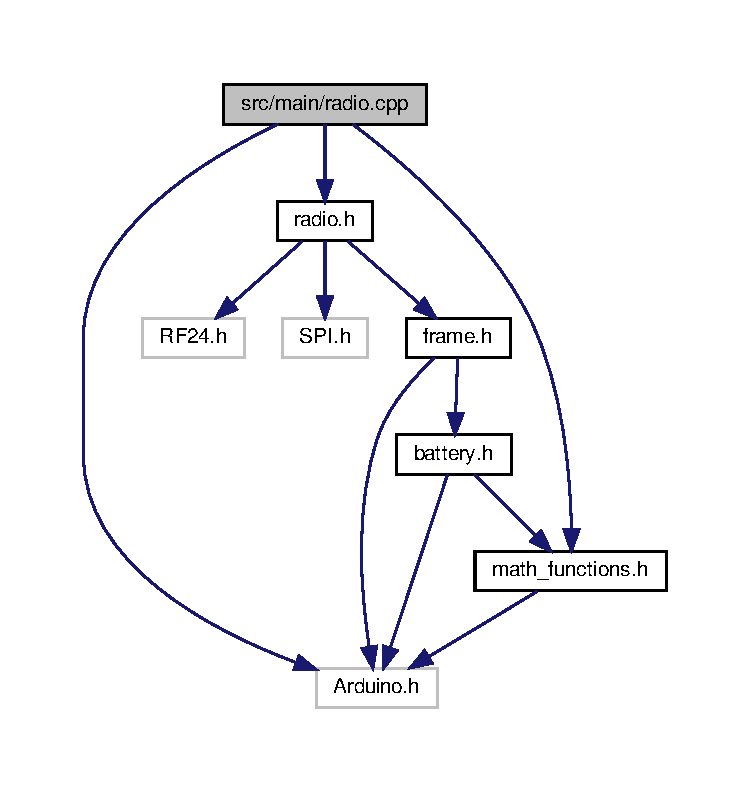
\includegraphics[width=350pt]{radio_8cpp__incl}
\end{center}
\end{figure}


\subsection{Detailed Description}
Definition of radio class. 

\begin{DoxyAuthor}{Author}
Valentin Mercy (\href{https://github.com/vmercy}{\tt https\+://github.\+com/vmercy}) 
\end{DoxyAuthor}
\begin{DoxyVersion}{Version}
0.\+1 
\end{DoxyVersion}
\begin{DoxyDate}{Date}
2020-\/11-\/24
\end{DoxyDate}
\begin{DoxyCopyright}{Copyright}
Copyright (c) 2020 
\end{DoxyCopyright}
